
\chapter{Power Series}

This chapter covers the following ideas. When you create your lesson plan, it should contain examples which illustrate these key ideas. Before you take the quiz on this unit, meet with another student out of class and teach each other from the examples on your lesson plan. 


\begin{enumerate}
\item Find and explain the use of Taylor polynomials, Talyor series, and Maclaurin series. Give examples for various common functions.
\item Explain how to use the ratio test to find the radius of convergence of a power series. 
\item Derive Euler's formula, and use it to explain why complex roots $a\pm bi$ of 2nd order ODE result in the solutions $e^{ax}\cos(bx)$ and $e^{ax}\sin(bx)$.
\item Explain how to differentiate, integrate, add, multiply, compose, and shift indices of power series.
\item Use the power series method to solve ODEs at ordinary points.
\end{enumerate}



%When you have finished this chapter, you will .....  Give the students a description of what they will learn, how it will benefit them, and why it is important in the future work that they do.  This needs to be done at the beginning of every chapter, as well as repeated at the end.  Make sure you start doing this when you go to revise your textbooks.

\section{Taylor Polynomials and Series} 

Recall that the tangent line to a function $f(x)$ at $x=c$ is a line through $(c,f(c))$ with slope $f^\prime(c)$.  An equation of this line (obtained using the point-slope form $y-y_0 = m(x-x_0)$)is $y-f(c)= f^\prime(c)(x-c)$, or in slope intercept form $y=f(c)+f^\prime(c)(x-c)$.  The tangent line provides an approximation to the function for values of $x$ close to $c$. As $x$ gets far from $c$, the approximation gets worse. In this section our main goal is to learn how to create better approximations to a function, using polynomials. Calculators use these ideas to evaluate numbers such as $\pi, e,$ and $\ln 2$.

Rather than use a line to approximate a function, we could instead use a parabola, a cubic function, or a polynomial of any degree. If we use a parabola (which we will call $P_2(x)$) to approximate $f(x)$ at $x=0$, then we want the parabola to pass through $(0,f(0))$, have the same slope at $0$ as $f$, and have the same concavity at $0$ as $f$.  This means we need to satisfy the three equations $P_2(0)=f(0),P_2^\prime(0)=f^\prime(0),P_2^{\prime\prime}(0)=f^{\prime\prime}(0)$. Since $P_2(x)$ is a parabola, we can write $P_2(x)=a_0 + a_1 x+a_2 x^2$ for the three unknowns $a_0,a_1,a_2$. We now have three equations and three unknowns, so we solve this system of equations. Since $P_2(0)=f(0),$ we have $a_0+0+0 = f(0)$.  The derivative of $P_2$ is $P_2^\prime(x) = a_1+2a_2x$, which at $0$ needs to equal $f^\prime(0)$. This means $a_1+0 = f^\prime(0)$.  The second derivative is $P_2^{\prime\prime}(x)=2a_2$, and so we have $2a_2=f^{\prime\prime}(0)$.  From these three equations we find that the coefficients of the parabola are $a_0=f(0), a_1=f^\prime(0),$ and $\ds a_2=\frac{f^{\prime\prime}(0)}{2}$, which means that $\ds P_2(x) = f(0)+f^\prime(0)x+\frac{f^{\prime\prime}(0)}{2}x^2.$ If we had instead used a cubic function, we would have found that $\ds P_3(x) = f(0)+f^\prime(0)x+\frac{f^{\prime\prime}(0)}{2}x^2+\frac{f^{\prime\prime\prime}(0)}{3\cdot 2}x^3$, where $\ds a_3 =  \frac{f^{\prime\prime\prime}(0)}{3\cdot 2}$.  For a degree 4 polynomial, we would have $\ds a_4=\frac{f^{\prime\prime\prime\prime}(0)}{4\cdot 3\cdot 2}$. In general, we find that $a_n = \frac{f^{(n)}(0)}{n!}$, where $n!=n(n-1)\cdots 3\cdot 2\cdot 1$ is called the factorial function. Using summation notation, we can write $\ds P_n(x) = \sum_{m=0}^{n}\frac{f^{(m)}(0)}{m!}x^m$.  This is called the Taylor polynomial of degree $n$ centered at $x=0$ of $f(x)$. If we want to approximate a function at a point other than 0, say $x=c$, then a similar calculation shows that $\ds P_n(x) = \sum_{m=0}^{n}\frac{f^{(m)}(c)}{m!}(x-c)^m$. If we let $m\to \infty$, the result is called a Taylor series (an infinite sum of terms). When we center our Taylor polynomials at $x=0$, the Taylor Series is called a MacLaurin series. Let's look at some examples.

The function $f(x)=\frac{1}{1-x}$ has as its first three derivatives $f^\prime(x) = \frac{1}{(1-x)^2}, f^{\prime\prime}(x) = \frac{2}{(1-x)^3},f^{(3)}(x) = \frac{3\cdot 2}{(1-x)^4}$.  It should become apparent that the $m$th derivative is $f^{(m)}(x) =  \frac{m!}{(1-x)^{m+1}}$.  Evaluating each of these functions at $x=0$, we see that $f(0)=f^{(0)}(0)=1, f^\prime(0)=1, f^{(2)}(0)=2!,f^{(3)}(0)=3!,\ldots, f^{(m)}(0)=m!,\ldots$. To obtain the coefficient $a_m$, we divide by $m!$ to obtain $a_m=1$ for all $m$.  Hence we see that the Taylor polynomials for $f(x)=\frac{1}{1-x}$ are $P_1(x) = 1+x, P_2=1+x+x^2,P_3=1+x+x^2+x^3,\ldots,\ds P_n = \sum_{m=0}^n x^m$. The calculations above for $f(x)=1/(1-x)$ can be organized into a table as shown below:
\begin{center}
\begin{tabular}{|c|c|c|c|c|}\hline
$m$ & $f^{(m)}(x)$ & $f^{(m)}(0)$ & $a_m=f^{(m)}(0)/m!$  & $a_m x^m$
\\\hline
$0$ & $(1-x)^{-1}$ & $1$ & $1/0!$ & $1$
\\\hline
$1$ & $(-1)(1-x)^{-2}(-1)$ & $1$ & $1/1!$ & $x$
\\\hline
$2$ & $(-1)(-2)(1-x)^{-3}(-1)^2$ & $2$ & $2/2!=1$ & $x^2$
\\\hline
$3$ & $(-1)(-2)(-3)(1-x)^{-3}(-1)^2$ & $3!$ & $3!/3!=1$ & $x^3$
\\\hline
$\vdots$ & $\vdots$ & $\vdots$ & $\vdots$ & $\vdots$
\end{tabular}
\end{center}
Once you have created this table, you can obtain a Taylor polynomial of any degree by summing the terms on the right of the table. The third degree Taylor polynomial is $P_3(x) = 1+x+x^2+x^3$. The Taylor series centered at $x=0$ (called the MacLaurin series) is $1+x+x^2+x^3+\cdots+x^n+\cdots = \sum_{m=0}^\infty x^m$.

Let's use the table format to find the 6th degree Taylor polynomial for $f(x)=\cos x$, centered at $x=0$.
\begin{center}
\begin{tabular}{|c|c|c|c|c|}\hline
$m$ & $f^{(m)}(x)$ & $f^{(m)}(0)$ & $a_m=f^{(m)}(0)/m!$  & $a_m x^m$
\\\hline
$0$ & $\cos x$ & $1$ & $1/0!=1$ & $1$
\\\hline
$1$ & $-\sin x$ & $0$ & $0/1!=0$ & $0$
\\\hline
$2$ & $-\cos x$ & $-1$ & $-1/2!$ & $-\frac{1}{2!}x^2$
\\\hline
$3$ & $\sin x$ & $0$ & $0/3!=0$ & $0$
\\\hline
$4$ & $\cos x$ & $1$ & $1/4!$ & $\frac{1}{4!}x^4$
\\\hline
$5$ & $-\sin x$ & $0$ & $1/5!=0$ & $0$
\\\hline
$6$ & $-\cos x$ & $-1$ & $-1/6!$ & $-\frac{1}{6!}x^6$
\\\hline
\end{tabular}
\end{center}
Summing the right column give the 6th degree Taylor polynomial as $P_6(x) = 1-\frac{1}{2}x^2 +\frac{1}{4!}x^4-\frac{1}{6!}x^6$.  Notice that $\frac{1}{6!}$ is extremely small, so the 6th order term doesn't change the value of $P_6(x)$ much for small values of $x$. 

What if we want to center the Taylor polynomial at a point other than zero. The table format below illustrates this for the 3rd degree Taylor polynomial of $f(x)=\sin x$, centered at $x=\pi$.
\begin{center}
\begin{tabular}{|c|c|c|c|c|}\hline
$m$ & $f^{(m)}(x)$ & $f^{(m)}(\pi)$ & $a_m=f^{(m)}(\pi)/m!$  & $a_m (x-\pi)^m$
\\\hline
$0$ & $\sin x$ & $0$ & $0/1!=0$ & $0$
\\\hline
$1$ & $\cos x$ & $-1$ & $-1/1!$ & $-\frac{1}{1!}(x-\pi)^1$
\\\hline
$2$ & $-\sin x$ & $0$ & $0/2!=0$ & $0$
\\\hline
$3$ & $-\cos x$ & $1$ & $1/3!$ & $\frac{1}{3!}(x-\pi)^3$
\\\hline
\end{tabular}
\end{center}
Summing the last column means the 3rd degree Taylor polynomial centered at $x=\pi$ is $P_3(x) = -\frac{1}{1!}(x-\pi)^1 + \frac{1}{3!}(x-\pi)^3$.

The graphs of several Taylor polynomials centered at $x=0$ for the functions $e^x, \frac{1}{1-x},\cos x$, and $\sin x$ are shown below. The higher the order of the polynomial, the closer it is to the actual function.
\newcommand{\mywidth}{1.3in}
\begin{center}
\begin{tabular}{cccc}
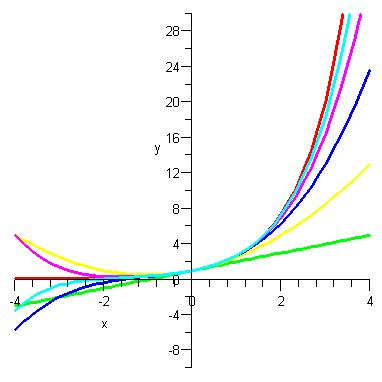
\includegraphics[width=\mywidth]{08-Power-Series/PowerSeries/taylore}&
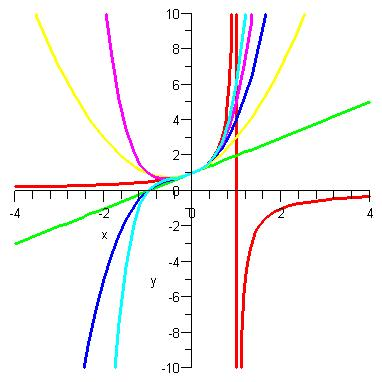
\includegraphics[width=\mywidth]{08-Power-Series/PowerSeries/taylor1}&
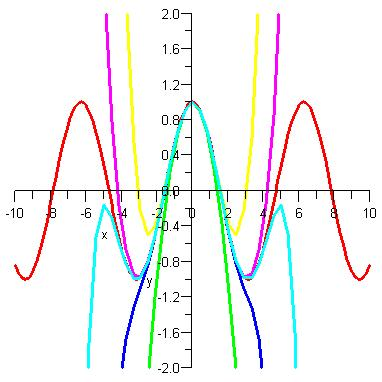
\includegraphics[width=\mywidth]{08-Power-Series/PowerSeries/taylorc}&
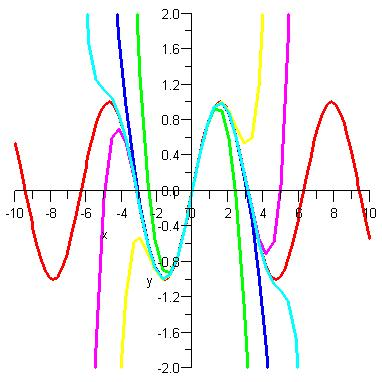
\includegraphics[width=\mywidth]{08-Power-Series/PowerSeries/taylors}
\\
$f(x)=e^x$&
$f(x)=\frac{1}{1-x}$&
$f(x)=\cos x$&
$f(x)=\sin x$
\end{tabular}
\end{center}
As you increase the degree of a Taylor polynomial, you should expect to see that your accuracy of approximating a function increases. This is true for $\cos x, \sin x, e^x,$ polynomials, and combination of these functions obtained through addition, subtraction, or multiplication. You can also divide any two of these function and still obtain good approximations, but vertical asymptotes pose a problem. 

The function $\frac{1}{1-x}$ has a vertical asymptote at $x=1$.  When we create Taylor polynomials centered at $x=0$, those polynomials follow the function up the left hand side of the vertical asymptote, causing the polynomials to tend toward infinity at $x=1$ as you increase the degree of the polynomial.  In the picture above, none of the polynomials do a good job of approximating the function to the right of $x=1$. Also, none of the functions do a good job of approximating the function to the left of $x=-1$. This is because Taylor polynomials are symmetric about where they are centered. When approximations break down on one side, they break down on the other side as well. We can only obtain useful approximations of $1/(1-x)$ for values of $x$ in the interval $(-1,1)$. The center of this interval is $x=0$, where we centered our Taylor polynomial. The distance from the center $x=0$ to the asymptote at $x=1$ is called our radius of convergence, and the interval of convergence $(-1,1)$ is obtained by moving 1 unit (the radius) to the right and left of 0 (the center).

%What happens if we change where we center our Taylor polynomial? When creating Taylor polynomials of increasing degree for $f(x) = 1/(1-x)$ centered at $x=-2$, the polynomials will do a great job of approximating the function until it reaches the asymptote at $x=1$.  Since the asymptote is 3 units away from $x=-2$ (where we centered the polynomial), our Taylor polynomials will produce increasing better approximations for any value of $x$ which is less than 3 units from $-2$, namely any $x$ in the interval $(-5,1)$. The number $3$ is our radius of convergence, and the interval $(-5,1)$ is our interval of convergence.
%
%There are vertical asymptotes for $\frac{1}{(x+4)(x-5)}$ at $-4$ and $5$. Taylor polynomials centered at $x=3$ produce useful approximations on an interval of radius 2 (the closer asymptote is at $x=5$ which is 2 units away), which means that as long as $x$ is in the interval $(1,5)$, you can use increasing larger Taylor polynomials centered at $x=3$ to make approximations good approximations. If instead you center the polynomials at $x=-1$, then the closest asymptote is at $x=-4$. This means the radius is $3$ and approximations can be made on the interval $(-4,2)$.  
%
%In math 316 you will learn about infinite sums of polynomials, and learn how to compute the radius of convergence using a tool called the ratio test. Taylor polynomials sometimes provide the only method known to numerically handle functions which are not polynomials (or quotients of polynomials). 





\subsection{Radius of convergence}
The Taylor series of a function involves adding infinitely many terms.  In some cases, the infinite sum will converge to a finite number. In other cases, the infinite sum will diverge. As an example, the Taylor series for $f(x) = \frac{1}{1-x}$ is $\ds  \sum_{m=0}^\infty x^m$. If $x=\frac{1}{2}$, then the series becomes $1+\frac{1}{2}+\frac{1}{4}+\frac{1}{8}+\frac{1}{16}+\cdots=2 = \frac{1}{1-1/2}$. We say this infinite sum converges to 2 because it gets closer and closer to 2 as you add more and more terms. Notice that the Taylor series actually converges to value of the function at $x=\frac{1}{2}$.  However, if you let $x=3$, then the series is $1+3+9+27+81+\cdots$ which diverges. In general, if a Taylor series converges at $x=c$, it will converge to $f(c)$. For this reason, we often write $\frac{1}{1-x} = \sum_{m=0}^\infty x^m$, and put an equal sign between the function and it's Taylor series.  However this equality sign will only hold if the series on the right converges. The infinite sum $\sum_{m=0}^\infty x^m$ is very closely related to the improper integral $\int_0^\infty x^m dm = \frac{x^m}{\ln x}\big|_{m=1}^\infty = \lim_{b\to\infty}\frac{x^b}{\ln x} - \frac{1}{\ln x}$. This improper integral converges if $0\leq x\leq 1$, and diverges otherwise. This integration fact can be used to show that sums of integer powers of $x$ converge if $|x|\leq 1$, and diverge if $|x|\geq 1$. We will use this fact to develop a powerful test called the ratio test which allows us to tell for which $x$ a power series will converge. 

For a series $\sum_{m=0}^\infty b_m$, the limit $\ds r=\lim_{m\to\infty}\frac{|b_{m+1}|}{|b_m|}$ compares how quickly a series grows.  Provided the limit $r$ exists, the series is comparable in growth to the series $\sum_{m=0}^\infty r^m$ which converges if $r\leq 1$ and diverges if $r>1$. A careful detailed analysis of this idea would require us to learn the Integral Test, absolute convergence, and comparison tests for series.  For our class, we will just use the fact that if $r<1$, then a series converges. For a Taylor series $\sum_{m=0}^\infty a_m (x-x_0)^m$ to converge, we need to satisfy the inequality $\lim_{m\to\infty}\frac{|a_{m+1}(x-x_0)^{m+1}|}{|a_m (x-x_0)^m|}<1$, or $\lim_{m\to\infty}\frac{|a_{m+1}|}{|a_m|}|x-x_0|<1$, or $|x-x_0|<1/ \lim_{m\to\infty}\frac{|a_{m+1}|}{|a_m|}$. We call the quantity $R=1/ \lim_{m\to\infty}\frac{|a_{m+1}|}{|a_m|}$ the radius of convergence of the power series because for $|x-x_0|<R$ the series converges. This formula for radius of convergence is handy if the series does not skip powers of $x$, however we return to the limit $\ds r=\lim_{m\to\infty}\frac{|b_{m+1}|}{|b_m|}<1$ to find the radius of convergence if the power series skips powers of $x$. In any case, a power series will have one of these three possible cases for it's radius of convergence: (1) $R=0$, so that the series only converges if $x=x_0$, (2) $R=\infty$, so that the series converges for all $x$ which is extremely nice, or (3) $R>0$, so that the series converges for $|x-x_0|<R$.

The series $\frac{1}{1-x}= \sum_{m=0}^\infty x^m$ has radius of convergence $\ds R=1/\lim_{m\to\infty}\frac{|1|}{|1|} = 1$, so if $|x|<1$ the series converges.  For the function $e^x = \sum_{m=0}^\infty \frac{x^m}{m!}$, the radius of convergence is $\ds R=1/\lim_{m\to\infty}\frac{|1/(m+1)!|}{|1/m!|} =1/\lim_{m\to\infty}\frac{m}{m+1} =\infty$ which means that the Taylor series for $e^x$ converges for all $x$. We have the series $\cos x = \sum_{m=0}^\infty \frac{1}{(2m)!} x^{2m}$ which skips powers of $x$.  Hence we solve $\ds \lim_{m\to\infty}\frac{|x^{2(m+1)}/(2(m+1))!|}{| x^{2m}/(2m)!|}<1$ which is equivalent to $|x^2|\lim_{m\to\infty}\frac{(2m)!}{ (2m+2)(2m+1)(2m)!}<1$ or $0<1$ which is always true so the radius of convergence is $\infty$ and the Taylor series converges for all $x$.  You should show that this is true for $\sin x$ as well. 

Let's find the radius of convergence of the power series $\ds\sum_{n=0}^\infty \frac{(3n+2)(-5)^n}{(n+1)(7n^2+3)2^{3n+1}}x^{2n}$.  We compute $a_{n+1} = \frac{(3(n+1)+2)(-5)^{n+1}}{((n+1)+1)(7(n+1)^2+3)2^{3(n+1)+1}}x^{2(n+1)}$.  Dividing by $a_n$ can get ugly unless we organize our work, for example by placing common terms directly above and below each other as shown below.
\begin{align*}
\left|\frac{a_{n+1}}{a_n}\right| 
&=  
\left|\begin{array}{c|c|c|c|c|c}
(3(n+1)+2)&(-5)^{n+1}&(n+1)&(7n^2+3)&2^{3n+1}&x^{2(n+1)}\\\hline
(3n+2)&(-5)^n&((n+1)+1)&(7(n+1)^2+3)&2^{3(n+1)+1}&x^{2n}
\end{array}\right|\\
&=\left|\begin{array}{c|c|c|c|c|c}
(3n+5)&(-5)^{n}(-5)&(n+1)&(7n^2+3)&2^{3n}2&x^{2n}x^2\\\hline
(3n+2)&(-5)^n&(n+2)&(7(n+1)^2+3)&2^{3n}2^{4}&x^{2n}
\end{array}\right|\\
&=\left|\begin{array}{c|c|c|c|c|c}
(3n+5)&(-5)&(n+1)&(7n^2+3)&1&x^2\\\hline
(3n+2)&1&(n+2)&(7(n+1)^2+3)&2^{3}&1
\end{array}\right|
\end{align*}
Recall that the limit of a product can be found by computing each individual limit and the multiplying the result together.  Also, the limit as $n\to \infty$ of a quotient of two polynomials of the same degree is precisely the quotient of their leading coefficients.  This means we can compute 
$\ds\lim_{n\to\infty}\frac{(3n+5)}{(3n+2)} = 1 $, 
$\ds\lim_{n\to\infty}\frac{(n+1)}{(n+2)} = 1 $, and 
$\ds\lim_{n\to\infty}\frac{(7n^2+3)}{(7(n+1)^2+3)} = 1$, which gives 
$$\lim_{n\to\infty}
\left|\begin{array}{c|c|c|c|c|c}
(3n+5)&(-5)&(n+1)&(7n^2+3)&1&x^2\\\hline
(3n+2)&1&(n+2)&(7(n+1)^2+3)&2^{3}&1
\end{array}\right| = \left|1(-5)(1)(1)\left(\frac{1}{8}\right)x^2\right| = \frac{5}{8}x^2.$$ 
We then solve the equation $\frac{5}{8}x^2<1$ for $x$ to obtain $|x|\leq\sqrt{\frac{8}{5}}$, so the radius of convergence is $\sqrt{\frac{8}{5}}$.

\subsection{Euler's Formula}
We now show $e^{ix}=\cos x+i\sin x$.  We know $\ds e^x = \sum_{m=0}^\infty\frac{1}{m!}x^m$ for all $x$, and it can be shown that this formula is valid as well for all complex numbers.  If we replace $x$ with $ix$, then we obtain $\ds e^{ix} = \sum_{m=0}^\infty\frac{1}{m!}(ix)^m$.  The powers of $i$ satisfy $i^0=1, i^1=i, i^2=-1, i^3=-i, i^4=1, i^5=i$, and cycle through the numbers $1,i,-1,-i$.  Hence we have for all $x$ Euler's formula
\begin{align*}
e^{ix} 
&= 1+ix-\frac{1}{2!}x^2-i\frac{1}{3!}x^3+\frac{1}{4!}x^4+i\frac{1}{5!}x^5-\frac{1}{6!}x^6-i\frac{1}{7!}x^7+\cdots\\
&= \left(1-\frac{1}{2!}x^2+\frac{1}{4!}x^4-\frac{1}{6!}x^6+\cdots\right)
+i\left(x-\frac{1}{3!}x^3+\frac{1}{5!}x^5-\frac{1}{7!}x^7+\cdots\right)\\
&= \left(\sum_{m=0}^\infty \frac{(-1)^m}{(2m)!}x^{2m}\right)
+i\left(\sum_{m=0}^\infty \frac{(-1)^m}{(2m+1)!}x^{2m+1}\right)\\
&= \cos(x)+i\sin(x).
\end{align*} 
%This means that $e^{(\alpha+\beta i)x} = e^{\alpha x}e^{\beta x i} = e^{\alpha x}(\cos\beta x +i\sin\beta x)$. This is Euler's formula. 

Who cares?  Well, if the roots of the second order ODE $my^{\prime\prime}+cy^\prime+ky=0$ are complex, i.e. $\lambda=a\pm b i$, then $y_1=e^{a x+ b ix} =e^{a x}(\cos b x+ i\sin b x)$ and $y_2=e^{a x-b i x}=e^{a x}(\cos (-bx)+i\sin(-b x)) = e^{a x}(\cos b x-i\sin b x)$ are two complex solutions of the ODE (recall that $\cos (-x)=\cos (x)$ [cosine is an even function] and $\sin(-x)=-\sin x$ [sine is an odd function]). The superposition principle for ODEs says that linear combinations are solutions, so $\frac{y_1+y_2}{2} = e^{a x}\cos b x$ and $\frac{y_1-y_2}{2i} = e^{a x}\sin b x$ are two real solutions.  This is why we use $e^{a x}\cos b x$ and $e^{a x}\sin b x$ as solutions when the roots of the characteristic equation are imaginary.

\section{Power Series}
\subsection{Notation and Calculus}
Rather than starting with a function $f(x)$ and calculating the Taylor series, we now reverse the process.  We will define a power series centered at $x=c$ to be an expression of the form $f(x) = \sum_{m=0}a_m (x-c)^m$, and the domain of $f$ is all $x$ for which the series converges. We will almost always center our power series at $x=0$, so we write $f(x) = \sum_{m=0}a_m x^m$. The radius of convergence is still computed the same. 
If the power series has a positive or infinite radius of convergence when centered at $x=c$, then we say that the function $f(x)= \sum_{m=0}a_m (x-x_0)^m$ is \textbf{analytic} at $c$. 

If a power series $f(x)= \sum_{m=0}a_m (x-x_0)^m$ has a finite radius of convergence, then we can differentiate and integrate the power series term by term. The resulting power series $f^\prime (x) = \sum_{m=0}m a_m (x-x_0)^{m-1}=\sum_{m=1}m a_m (x-x_0)^{m-1} $ and $\int f(x)dx = C+\sum_{m=0}\frac{a_m}{m+1} (x-x_0)^{m+1}$ have the same radius of convergence as $f$.  If two power series centered at the same point both converge at $x$, then you can add them (by adding their coefficients), and multiply them (using the distributive laws of multiplication). In addition, you can compose power series, though this may change the radius of convergence.  The most common composition is to replace $x$ with $a(x)^k$ for some constants $a$ and $k$. 

\subsection{Examples}
Since $\ds \frac{1}{1-x} = \sum_{m=0}^\infty x^m$ has radius of convergence $R=1$, we can differentiate and obtain $\ds \frac{1}{(1-x)^2} = \sum_{m=1}^\infty m x^{m-1} = 1+2x+3x^2+4x^3+\cdots$, which has radius of convergence $R=1$ as well.  Replacing $x$ with $x=-x$ gives $\ds \frac{1}{1+x} = \sum_{m=0}^\infty (-1)^m x^m = 1-x+x^2-x^3+x^4+\cdots$. Replacing $x$ with $-x^2$ gives $\ds \frac{1}{1+x^2} = \sum_{m=0}^\infty (-1)^m x^{2m} = 1-x^2+x^4-x^6+x^8+\cdots$. Integration of $\frac{1}{1+x^2}$ gives (notice that $\arctan(0)=0$ so the constant is zero) $\arctan x = \ds \sum_{m=0}^\infty \frac{(-1)^m}{2m+1} x^{2m+1} = x-\frac13x^3+\frac15x^5-\frac17x^7+\frac19x^9+\cdots$, with radius of convergence $R=1$. For homework, find the power series of $\ln|1+x|,\ln\left|\frac{1+x}{1-x}\right|,\frac{x}{1+x^2},$ and a few others that you can find any any calculus textbook.  

To find the radius of convergence of the power series $\arctan 2x = \ds \sum_{m=0}^\infty \frac{(-1)^m}{2m+1} (2x)^{2m+1}$, we notice that powers of $x$ are skipped. So we solve 
$\ds \lim_{m\to\infty}\frac{|(2x)^{2(m+1)+1}/(2(m+1)+1)|}{|(2x)^{2m+1}/2m+1|}<1$, 
which is equivalent to 
$\ds \lim_{m\to\infty}\frac{(2x)^{2m+3}(2m+1)}{(2x)^{2m+1}(2m+3)}<1$ or
$\ds (2x)^2 \lim_{m\to\infty}\frac{(2m+1)}{(2m+3)}<1$. Taking limits gives $(2x)^2<1$ or $|2x|<1$ which means $|x|<\frac{1}{2}$. Hence the radius of convergence is 1/2.  

The radius of convergence of the power series $f(x) = \sum_{m=0}\frac{m}{8^m} x^{3m}$ can be found by solving 
$\ds \lim_{m\to\infty}\frac{|(m+1)x^{3(m+1)}/8^{m+1}|}{|mx^{3m}/8^{m}|}<1$. The left side simplifies as 
$\ds \lim_{m\to\infty}\frac{(m+1)x^{3m+3)}/8^{m}8}{mx^{3m}/8^{m}} = |x^3|\lim_{m\to\infty}\frac{(m+1)/8}{m} =|x^3/8|$.  The solution to $|x^3/8|<1$ is $|x^3|<8$ or $|x|<2$.  Hence the radius of convergence is $2$. Notice that we know this power series converges for $|x|<2$, even though we do not know what it converges to.   

\subsection{Shifting Indices}
Often we will find it necessary to shift the indices of a power series. The series $\ds\sum_{m=1}^\infty m a_m x^{m-1}$ is equivalent (letting $s=m-1$ or $m=s+1$) to the series $\ds\sum_{s=0}^\infty (s+1)a_{s+1} x^{s}$. The variables $m$ and $s$ are just ``dummy'' variables used as a place holder.  They can be changed as much as you want, just as you can change the variable of integration in an integration problem.  The change $s=m-1$ is called shifting the indices of a series.  The series $\ds\sum_{m=3}^\infty \frac{m+1}{m-2} x^{m-3}$ can be shifted to start at $0$ by letting $s=m-3$, and then we write $\ds\sum_{s=0}^\infty \frac{s+4}{s+1} x^{s}$, since $m=s+3$ (just replace each $m$ with $s+3$ and the result follows). 












\section{Series Solutions to ODEs}


Recall that a function which can be represented by a power series centered at $c$ with a positive radius of convergence is said to be analytic at $c$. It can be shown that the 2nd order ODE $h(x)y^{\prime\prime}+p(x)y^\prime+q(x)y=r(x)$ has a power series solution centered at $c$ if $h,p,q,r$ are all analytic at $c$ and $h(x_0)\neq 0$. Alternatively, if we divide by $h(x)$, then the 2nd order ODE $y^{\prime\prime}+a(x)y^\prime+b(x)y=c(x)$ has a power series solution centered at $x=c$ if $a(x),b(x),c(x)$ are all analytic at $x=c$.  In this case we call $x=c$ an ordinary point of the ODE.  The radius of convergence of the power series solution we obtain for $y(x)$ will be at least as big as the smallest radius of convergence of $a(x),b(x),c(x)$. This is the general theory which motivates everything else we do with regards to series solutions to ODEs. 

The power series method essentially requires that you (1) write $\ds y=\sum_{n=0}^\infty a_n x^n$, (2) take derivatives $\ds y=\sum_{n=0}^\infty n a_n x^{n-1}$ and $\ds y=\sum_{n=0}^\infty n(n-1) a_n x^{n-2}$, (3) replace each function or derivative in your ODE with the appropriate power series (computing MacLaurin series of functions which occur) (4) shift the indices on each sum to obtain a recurrence relation for the unknown constants $a_n$, and then (5) solve the recurrence relation for the largest $a_n$ and use this relation to generate the constants.  The following 4 examples illustrate how to find solutions using the power series method. Some of these problems you already can solve without power series methods, however we will start with simpler problems to which you already know the answer before we venture into new problems.

Consider the ODE $y^\prime=ky$.  Let $\ds y=\sum_{m=0}^\infty a_m x^m$.  Then we compute
$\ds y^\prime 
= \sum_{m=0}^\infty m a_m x^{m-1} 
= \sum_{m=1}^\infty m a_m x^{m-1} 
$. Notice that we can start at $m=1$ instead of $m=0$ because when you put $m=0$ into the sum you get zero, so why not just start one term later and skip the 0 term.
Inserting these series into the ODE gives 
$\ds \sum_{m=1}^\infty m a_m x^{m-1}=k\sum_{m=0}^\infty a_m x^m = \sum_{m=0}^\infty ka_m x^m$. For this equality to hold, we must have the coefficient of each power $x$ equal on each side of the equation.  To simplify the calculations, we shift the indices on the power series on the left by letting $m-1=s$, and on the right by letting $m=s$.  This gives $\ds \sum_{s=0}^\infty (s+1) a_{s+1} x^{s}= \sum_{s=0}^\infty ka_s x^s$, which means that $(s+1) a_{s+1} = ka_s$ for all $s$.  This gives the recurrence relation $a_{s+1}=\frac{ka_s}{(s+1)}$.  The variable $a_0$ can be chosen to be anything we want, but then $a_1=\frac{ka_0}{1},a_2=\frac{k^2a_0}{2!},a_3=\frac{k^3a_0}{3!}, a_m=\frac{k^ma_0}{m!}$.  So we have our solution as $$y(x) = a_0+a_0\frac{k}{1!}x^1+a_0\frac{k^2}{2!}x^2+\cdots = a_0\left(1+\frac{1}{1!}(kx)^1 + \frac{1}{2!}(kx)^2+\cdots\right) = a_0 \sum_{m=0}^\infty \frac{1}{m!}(kx)^m= a_0 e^{kx},$$ where the last equality comes because we recognize that this is the Maclaurin series of $e^{kx}$.

Consider the ODE $y^\prime=xy$. Let $\ds y=\sum_{m=0}^\infty a_m x^m$.  Then we compute
$\ds y^\prime 
= \sum_{m=0}^\infty m a_m x^{m-1} 
= \sum_{m=1}^\infty m a_m x^{m-1} 
$ (again we start at 1 because $m=0$ just gives us zero).
Inserting these series into the ODE gives 
$\ds \sum_{m=1}^\infty m a_m x^{m-1}=x\sum_{m=0}^\infty a_m x^m = \sum_{m=0}^\infty a_m x^{m+1}$.
Writing out the first few terms, we have $$1a_1x^0+2a_2x^1+3a_3x^2+4a_4x^3+\cdots = a_0x^1+a_1x^2+a_2x^3+a_3x^4.$$
Since $x^0$ appears only on the left side of the equation, we have $a_1=0$.  Hence the left side can be written $\ds \sum_{m=2}^\infty m a_m x^{m-1}$. We shift indices by letting $s=m-1$ ($m=s+1$) on the left side and $s=m+1$ on the right side.  This gives 
$\ds \sum_{s=1}^\infty (s+1) a_{s+1} x^{s}=\sum_{s=1}^\infty a_{s-1} x^{s}$. Equating the coefficients of $x^s$ (for $s\geq 1$) gives $(s+1) a_{s+1} = a_{s-1}$, or $a_{s+1} = \frac{a_{s-1}}{(s+1)}$ for $s\geq 1$.  For $s=1,2,3,4,5,6,\ldots$ we have $a_{2} = \frac{a_{0}}{(2)},a_{3} = \frac{a_{1}}{(3)}=0, a_{4} = \frac{a_{2}}{(4)} =\frac{a_{0}}{(2\cdot 4)}, a_5=0, a_6=\frac{a_{0}}{(2\cdot 4\cdot 6)} = \frac{a_{0}}{2^3 3!}, \ldots$.  Notice that $a_m=0$ for odd $m$, and $a_{2m}=\frac{a_{0}}{2^m m!}$.  If $m=0$, we can still write $a_{2m}=\frac{a_{0}}{2^m, m!}=a_0$, which means we can write $y=\sum_{m=0}^\infty \frac{a_{0}}{2^m m!}x^{2m} = a_0\sum_{m=0}^\infty \frac{1}{m!}\left(\frac{x^2}{2}\right)^{m} = a_0e^{x^2/2}$.


Now consider the ODE $y^{\prime\prime}+y=0$.  Let $\ds y=\sum_{m=0}^\infty a_m x^m$.  Then we compute 
$\ds y^\prime 
= \sum_{m=0}^\infty m a_m x^{m-1} 
= \sum_{m=1}^\infty m a_m x^{m-1} 
$ and 
$\ds y^{\prime \prime }
= \sum_{m=1}^\infty m(m-1) a_m x^{m-2} 
= \sum_{m=2}^\infty m(m-1) a_m x^{m-2} 
$ (we can start the second derivative at $m=2$ because putting $m=0$ or $m=1$ into the series gives 0).
Inserting these power series into the ODE gives $\sum_{m=2}^\infty m(m-1) a_m x^{m-2}+\sum_{m=0}^\infty a_m x^m=0$.  Shifting the indices on the first sum using $s=m-2$ (or $m=s+2$) and second sum using $m=s$ gives $\sum_{s=0}^\infty (s+2)(s+1) a_{s+2} x^{s}+\sum_{s=0}^\infty a_s x^s=0$. We need to have the sum of the coefficients of $x^s$ sum to zero, so we have $(s+2)(s+1) a_{s+2} + a_s=0$.  This means $a_{s+2} = -\frac{a_s}{(s+2)(s+1)}$ for $s\geq 0$.  This recurrence relation does not specify $a_0$ or $a_1$, so we have two constants we can choose arbitrarily.  For $s=0,1,2,3,\ldots$, we have $a_{2} = -\frac{a_0}{2!}, a_{3} = -\frac{a_1}{3!},a_{4} = \frac{a_0}{4!},a_{5} = \frac{a_1}{5!},a_{6} = -\frac{a_0}{6!},a_{7} = -\frac{a_1}{7!}\ldots$. The sign changes in groups of two, which suggests we should split the series into even and odd powers. This can be summarized as $a_{2m}=(-1)^m\frac{a_0}{(2m)!}$ and $a_{2m+1}=(-1)^m\frac{a_1}{(2m+1)!}$.  This means that the solution to the ODE is 
\begin{align*}
y(x) &= a_0+a_1x-a_0\frac{1}{2!}x^2-a_1\frac{1}{3!}x^3+a_0\frac{1}{4!}x^4+a_1\frac{1}{5!}x^5+\cdots \\
&=a_0\left(1-\frac{1}{2!}x^2+\frac{1}{4!}x^4+\cdots\right)+a_1\left(x-\frac{1}{3!}x^3+\frac{1}{5!}x^5+\cdots\right)\\
&= a_0\left(\sum_{m=0}^\infty \frac{(-1)^m}{(2m)!}x^{2m}\right)+a_1\left(\sum_{m=0}^\infty \frac{(-1)^m}{(2m+1)!}x^{2m+1}\right)\\
&= a_0\cos(x)+a_1\sin(x).\\
\end{align*}
The last equality can be discovered by recognizing that the series are the MacLaurin series for cosine and sine.


As our last example, consider the ODE
$y^{\prime\prime}+2xy^\prime+y=0$. Let $\ds y=\sum_{m=0}^\infty a_m x^m$. Then we compute 
$\ds y^\prime 
= \sum_{m=0}^\infty m a_m x^{m-1} 
= \sum_{m=1}^\infty m a_m x^{m-1} 
$ and 
$\ds y^{\prime \prime }
= \sum_{m=1}^\infty m(m-1) a_m x^{m-2} 
= \sum_{m=2}^\infty m(m-1) a_m x^{m-2} 
$.
Inserting these power series into the ODE and multiplying the middle series by 2x gives 
$$\sum_{m=2}^\infty m(m-1) a_m x^{m-2}+\sum_{m=1}^\infty 2m a_m x^{m} +y=\sum_{m=0}^\infty a_m x^m=0.$$ We shift the index on the first series by letting $s=m-2$ and $s=m$ for the last two.  This gives 
$$\sum_{s=0}^\infty (s+2)(s+1) a_{s+2} x^{s}+\sum_{s=1}^\infty 2s a_s x^{s} +\sum_{s=0}^\infty a_s x^s=0.$$ Notice that the second series starts at $s=1$ whereas the other two start at $s=0$.  Hence we look at the coefficients of $x^0$ separately than the rest of the coefficients.  We notice that $(2)(1)a_2 +a_0 = 0$, or $a_2=-a_0\frac{1}{2!}$.  For $s\geq 1$ we have $(s+2)(s+1) a_{s+2}+2s a_s+a_s =0$, or $ a_{s+2} = -a_s\frac{2s+1}{(s+2)(s+1)}$. The first few terms are $a_2=-a_0\frac{1}{2!}, a_3 = -a_s\frac{3}{(3)(2)}, a_4=a_0\frac{1\cdot 5}{4!},a_5=a_1\frac{3\cdot 7}{5!},a_6=-a_0\frac{1\cdot 5\cdot 9}{6!},-a_7=a_1\frac{3\cdot 7\cdot 11}{7!}$. Since the even and odd coefficients $a_m$ depend on $a_0$ and $a_1$, we write $a_{2m}=a_0(-1)^m \frac{1\cdot 5\cdot 9\cdots(4m-3)}{(2m)!}$ and $a_{2m+1}=a_1(-1)^m\frac{3\cdot 7\cdot 11\cdots(4m-1)}{(2m+1)!}$. Hence we have found a solution as 
\begin{align*}
y(x) &= a_0\left(1-{\frac {1}{2}}{t}^{2}+{\frac {5}{24}}{t}^{4}-{
\frac {1}{16}}{t}^{6}+{\frac {13}{896}}{t}^{8}+\cdots
 \right) +a_1\left(t-{\frac {1}{2}}{t}^{3}+{\frac {7}{40}}{t}^{5}-{
\frac {11}{240}}{t}^{7}+{\frac {11}{1152}}{t}^{9} +\cdots\right)\\
&= a_0\left(1+\sum_{m=1}^\infty (-1)^m \frac{1\cdot 5\cdot 9\cdots(4m-3)}{(2m)!}x^{2m} \right) +a_1\left(x+\sum_{m=1}^\infty (-1)^m\frac{3\cdot 7\cdot 11\cdots(4m-1)}{(2m+1)!}x^{2m+1} \right). 
\end{align*}
This is not a simple elementary function for which we know a power series. The radius of convergence is $R=\infty$.  We will learn how to express this function in terms of Bessel functions and Gamma functions when we start studying special functions in the next learning module.  Hence, we leave our solution in terms of a power series and cannot continue any further.

As you work problems in the homework, I want you to find general formulas for the $m$th coefficient $a_m$. Mathematica has code you can use to check if your answers are correct, as well as show you many of the steps in the computation. 

